\section{Solutions}

\subsection{Solutions to Possible/Impossible Questions}
	\begin{table}[!h]
		\centering
		\begin{tabular}{c@{\hspace{2.5em}}cp{0.75\textwidth}}
			possible & impossible & \\
			\specialrule{\lightrulewidth}{0.25em}{1.25em}
			\bubble & \dbubble & A matrix \(A \in \mathbb{R}^{m \times 2}\) whose solution set for the equation \(A\vec{x} = \vec{b}\) is the \(x_2\)
						       axis, and \(\vec{b} \ne \vec{0}\). \\[0.75em]
			\dbubble & \bubble & A matrix \(A \in\mathbb{R}^{m\times n}\) and the solution set of \(A\vec{x} = \vec{0}\) is \(\mathbb{R}^{n}\).\\[0.75em]
			\bubble & \dbubble & A matrix \(A\in\mathbb{R}^{m\times n}\) such that the solution set of the equation \(A\vec{x}=\vec{0}\) is empty.\\[0.75em]
			\dbubble & \bubble & A solution \(\vec{v}\) to the equation \(A \vec{v} = \vec{0}\) but none of the entries of \(\vec{v}\) is 0. \\[0.75em]
			\bubble & \dbubble & A matrix \(A\in\mathbb{R}^{2\times 3}\) where \(\vec{0}\) is the only solution to the equation \(A\vec{x}=\vec{0}\).\\[0.75em]
			\bottomrule
		\end{tabular}
	\end{table}

\subsection{Solutions to Short Answer Questions}
\begin{enumerate}
	\item \(\vec{x} = \begin{bmatrix}0 \\ 1\end{bmatrix}\) has to be a solution to \(A\vec{x} = \vec{0}\). Recall that 
		\[A\vec{x} = 0 \iff \vec{a}_1x_1 + \vec{a}_2 = \vec{0}.\] Set \(x_1 = 0\) and \(x_1 = 1\). We get that 
		\[(0)\vec{a}_1 + (1)\vec{a}_2 = \vec{0}.\]
		We see that the first column is therefore \emph{anything} and the second column is the zero vector. As you encounter more and more of these types of 
		questions, you'll start to do this \emph{instinctively}.

	\item The paramteric vector form for the solution set of the inhomogeouns equation is 
		\[\vec{x} = \begin{bmatrix}0 \\ 1/2\end{bmatrix} + t\begin{bmatrix}-3 \\ 1\end{bmatrix}, \quad t \in \mathbb{R}.\footnote{A lot of people got the
		paramterization \(\vec{x} = \begin{bmatrix}3/2 \\ 0\end{bmatrix} + t\begin{bmatrix}-3 \\ 1 \end{bmatrix}\). Don't panic! Both answers
		are correct. Remember, \(\vec{v}_p\) is \emph{one} of many particular solutions. If you have any questions on this, please create a post on Piazza.}\]
		The sketch would look like this.
		(Also, the graph for the solution set to the homogenous equation is shown as well. Note that the red line is translated
		up by a half, that's the \(\vec{v}_p\) in \(\vec{x} = \vec{v}_p + \vec{v}_n\)!)
		\begin{figure}[!h]
			\centering
			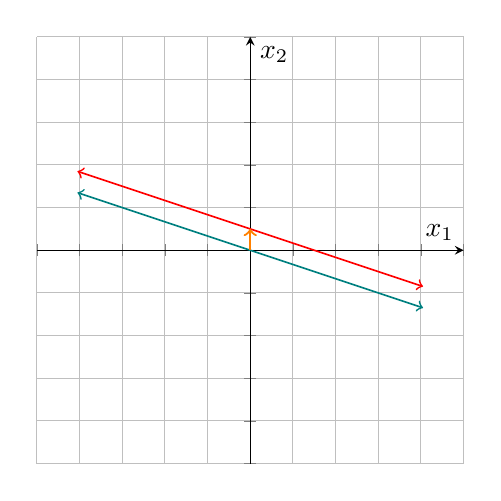
\begin{tikzpicture}
				\begin{axis}[
					height=7cm,
					width=7cm,
					axis lines = middle,
					xmin=-5, xmax=5, ymin=-5, ymax=5,
					xtick distance=1, ytick distance=1,
					xticklabels={}, yticklabels={,,},
					xlabel=\(x_1\), ylabel=\(x_2\),
					grid=major
				]
					\addplot[<->, red, semithick, domain=-1.35:1.35] ({-3 * x}, {0.5 + x});
					\addplot[<->, teal, semithick, domain=-1.35:1.35] ({-3 * x}, {x});
					\draw[->, orange, thick] (axis cs: 0, 0) -- (axis cs: 0, 0.5);
				\end{axis}
			\end{tikzpicture}
		\end{figure}

	\item We get a nontrivial solution once there is a free variable in the system corresponding to \(A\vec{x} = \vec{0}\). In order to ensure that the only solution is the
		trivial solution, find a 3-by-2 matrix that has \emph{no} free variables.
	
	\item Consider the case where the inhomogenous system is inconsistent.
\end{enumerate}